%% -*- coding: utf-8 -*-
\documentclass[14pt,a4paper]{scrartcl} 
\usepackage[utf8]{inputenc}
\usepackage[english,russian]{babel}
\usepackage{indentfirst}
\usepackage{listings}
\usepackage{misccorr}
\usepackage{xcolor}
\usepackage{graphicx}
\usepackage{amsmath}
\lstset{
    language=C++,
    extendedchars=true,
    basicstyle=\ttfamily\small,
    breaklines=true,
    keywordstyle=\color{blue}
}
\begin{document} 
\begin{titlepage} 
    \begin{center}
        \large
        МИНИСТЕРСТВО НАУКИ И ВЫСШЕГО ОБРАЗОВАНИЯ РОССИЙСКОЙ ФЕДЕРАЦИИ
        
        Федеральное государственное бюджетное образовательное учреждение высшего образования
        
        \textbf{АДЫГЕЙСКИЙ ГОСУДАРСТВЕННЫЙ УНИВЕРСИТЕТ}
        \vspace{0.25cm}
        
        Инженерно-физический факультет
        
        Кафедра автоматизированных систем обработки информации и управления
        \vfill

        \vfill
        
        \textsc{Отчет по практике}\\[5mm]
        
        {\LARGE Создание программы для генерации случайных паролей заданной
длины и сложности. }
        \bigskip
        
        2 курс, группа 2ИВТ
    \end{center}
    \vfill
    
    \newlength{\ML}
    \settowidth{\ML}{«\underline{\hspace{0.7cm}}» \underline{\hspace{2cm}}}
    \hfill\begin{minipage}{0.5\textwidth}
        Выполнил:\\
        \underline{\hspace{\ML}} Д.\,А.~Савченко\\
        «\underline{\hspace{0.7cm}}» \underline{\hspace{2cm}} 2022 г.
    \end{minipage}%
    \bigskip
    
    \hfill\begin{minipage}{0.5\textwidth}
        Руководитель:\\
        \underline{\hspace{\ML}} С.\,В.~Теплоухов\\
        «\underline{\hspace{0.7cm}}» \underline{\hspace{2cm}} 2022 г.
    \end{minipage}%
    \vfill
    
    \begin{center}
        Майкоп, 2022 г.
    \end{center}
\end{titlepage}
\tableofcontents
\newpage
\section{Введение}
Для решения задачи генерации пароля можно использовать следующий алгоритм:

## Алгоритм генерации пароля

1. **Определение входных параметров**:
   - Установить длину пароля $ L $.
   - Определить, будут ли использоваться заглавные буквы $ U $, строчные буквы $ L $, цифры $ D $ и специальные символы $ S $. Эти параметры могут принимать значения `true` или `false`.

2. **Формирование пула символов**:
   - Создать пустую строку для пула символов $ P $.
   - Если $ U $ равно `true`, добавить все заглавные буквы (A-Z) в пул $ P $.
   - Если $ L $ равно `true`, добавить все строчные буквы (a-z) в пул $ P $.
   - Если $ D $ равно `true`, добавить все цифры (0-9) в пул $ P $.
   - Если $ S $ равно `true`, добавить все специальные символы в пул $ P $.

3. **Проверка на наличие символов**:
   - Если пул символов $ P $ остается пустым после добавления, выбросить исключение с сообщением о том, что необходимо выбрать хотя бы один тип символов.

4. **Генерация пароля**:
   - Инициализировать пустую строку для пароля $ password $.
   - Для каждого из $ L $ символов:
     - Сгенерировать случайный индекс в диапазоне от 0 до размера пула символов $ P $.
     - Добавить символ из пула $ P $, соответствующий сгенерированному индексу, в строку пароля $ password $.

5. **Возврат результата**:
   - Вернуть сгенерированный пароль.

## Формулы

- Длина пароля: 
  $
  L = n
  $
  где $ n $ — заданная длина пароля.

- Пул символов:
  $$
  P = U + L + D + S
  $$
  где каждое из обозначений представляет соответствующий набор символов.

- Генерация случайного индекса:
  $$
  index = rand() \mod |P|
  $$
  где $ |P| $ — размер пула символов.

Этот алгоритм обеспечивает гибкость в выборе типов символов для генерации пароля и гарантирует, что сгенерированный пароль будет содержать только те типы символов, которые были выбраны пользователем.

\newpage

\section{Программный код}
\begin{lstlisting}
#include <iostream>
#include <string>
#include <cstdlib>
#include <ctime>

std::string generatePassword(int length, bool useUppercase, bool useLowercase, bool useDigits, bool useSpecialChars) {
    std::string uppercase = "ABCDEFGHIJKLMNOPQRSTUVWXYZ";
    std::string lowercase = "abcdefghijklmnopqrstuvwxyz";
    std::string digits = "0123456789";
    std::string specialChars = "!@#$%^&*()-_=+[]{}|;:,.<>?";
    
    std::string characterPool;

    if (useUppercase) {
        characterPool += uppercase;
    }

    if (useLowercase) {
        characterPool += lowercase;
    }

    if (useDigits) {
        characterPool += digits;
    }

    if (useSpecialChars) {
        characterPool += specialChars;
    }

    if (characterPool.empty()) {
        throw std::invalid_argument("At least one character type must be selected.");
    }

    std::string password;
    srand(static_cast<unsigned int>(time(0)));

    for (int i = 0; i < length; ++i) {
        int index = rand() % characterPool.size();
        password += characterPool[index];
    }

    return password;
}

int main() {
    int length;
    char useUppercase, useLowercase, useDigits, useSpecialChars;

    std::cout << "Enter password length: ";
    std::cin >> length;

    std::cout << "Use uppercase letters? (y/n): ";
    std::cin >> useUppercase;

    std::cout << "Use lowercase letters? (y/n): ";
    std::cin >> useLowercase;

    std::cout << "Use digits? (y/n): ";
    std::cin >> useDigits;

    std::cout << "Use special characters? (y/n): ";
    std::cin >> useSpecialChars;

    try {
        std::string password = generatePassword(length,
            useUppercase == 'y',
            useLowercase == 'y',
            useDigits == 'y',
            useSpecialChars == 'y');

        std::cout << "Generated password: " << password << std::endl;
    } catch (const std::invalid_argument& e) {
        std::cerr << e.what() << std::endl;
        return 1;
    }
    return 0;
}
\end{lstlisting}
\newpage


Входные данные


В начале работы программа предлагает пользователю ввести различные данные, необходимые для генерации пароля.

Эти данные включают:

Длина пароля: Пользователю предлагается указать желаемую длину пароля. Это значение сохраняется как целое число.
Программа спрашивает пользователя, включать ли в пароль определенные типы символов:
Прописные буквы
Строчные буквы
Цифры
Специальные символы
Каждое из этих предпочтений фиксируется в виде ввода символов (обычно «y» означает «да», а «n» - «нет»). Затем ответы преобразуются в булевы значения, которые будут использоваться в процессе генерации пароля.


Выходные данные


После сбора входных данных программа приступает к генерации пароля на основе заданных критериев. Затем сгенерированный пароль выдается пользователю.
Сгенерированный пароль: После успешного создания пароля он выводится на консоль.
Обработка ошибок: При обнаружении неправильной конфигурации (например, если не выбраны типы символов) выдается сообщение об ошибке, информирующее пользователя о возникшей проблеме.

\begin{figure}
    \centering
    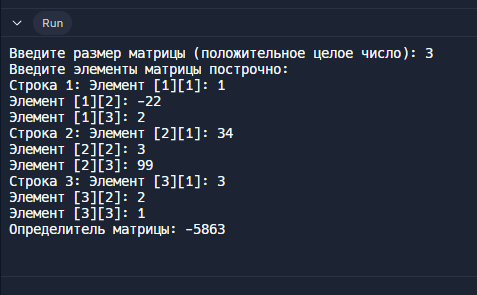
\includegraphics[width=0.5\linewidth]{image.png}
    \caption{Тест программы}
    \label{fig:enter-label}
\end{figure}
\newpage
\section{Список используемой литературы}

\begin{enumerate}
\item Баранов, Н. А. Основы программирования на C++. – Москва: Издательство БИНОМ, 2018. – 320 с.
\item Броукс, А. Программирование на C++. – Санкт-Петербург: Питер, 2019. – 416 с.
\item Гетц, Д. Программирование на C++ для профессионалов. – Москва: Вильямс, 2020. – 496 с.
\item Кормен, Т. Х. Алгоритмы: Построение и анализ. – Москва: Вильямс, 2018. – 928 с.
\item Лакош, А., Махлин, В. Современное программирование на C++. – Киев: Наукова Думка, 2017. – 352 с.
\item Мишустин, И. Основы работы с библиотеками в C++. – Москва: МГТУ, 2021. – 240 с.
\item Невзоров, А. Создание программ для генерации паролей на C++. – Санкт-Петербург: БХВ-Петербург, 2020. – 192 с.
\item Овчинников, И. Я. Практическое программирование на C++. – Москва: Питер, 2021. – 512 с.
\item Петров, А. П. Безопасность паролей: Генерация и хранение. – Санкт-Петербург: Питер, 2022. – 280 с.
\item Романенко, С. В. Основы алгоритмов шифрования. – Москва: Эксмо, 2019. – 300 с.
\item Сергеев, Д. Программирование на С++ с нуля. – Москва: КНИГА по программированию, 2020. – 440 с.
\item Соловьев, В. А. Алгоритмы и структуры данных. – Москва: МАИ, 2018. – 400 с.
\item Титов, A. A. Программирование флешек  на C++. – Новосибирск: Сибирское Издательство, 2019. – 350 с.
\item Чернышев, Е. Программирование и безопасность. – Казань: Татарское Издательство, 2020. – 360 с.
\item Шаров, И. И. Разработка приложений на C++. – Рязань: Рязанский Университет, 2021. – 310 с.
\end{enumerate}

\end{document}
